\section{Results}
\begin{figure*}[!ht]            % “*”→span both columns; [!t]→force it to the top
  \centering
  % first image, take roughly half the page width:
  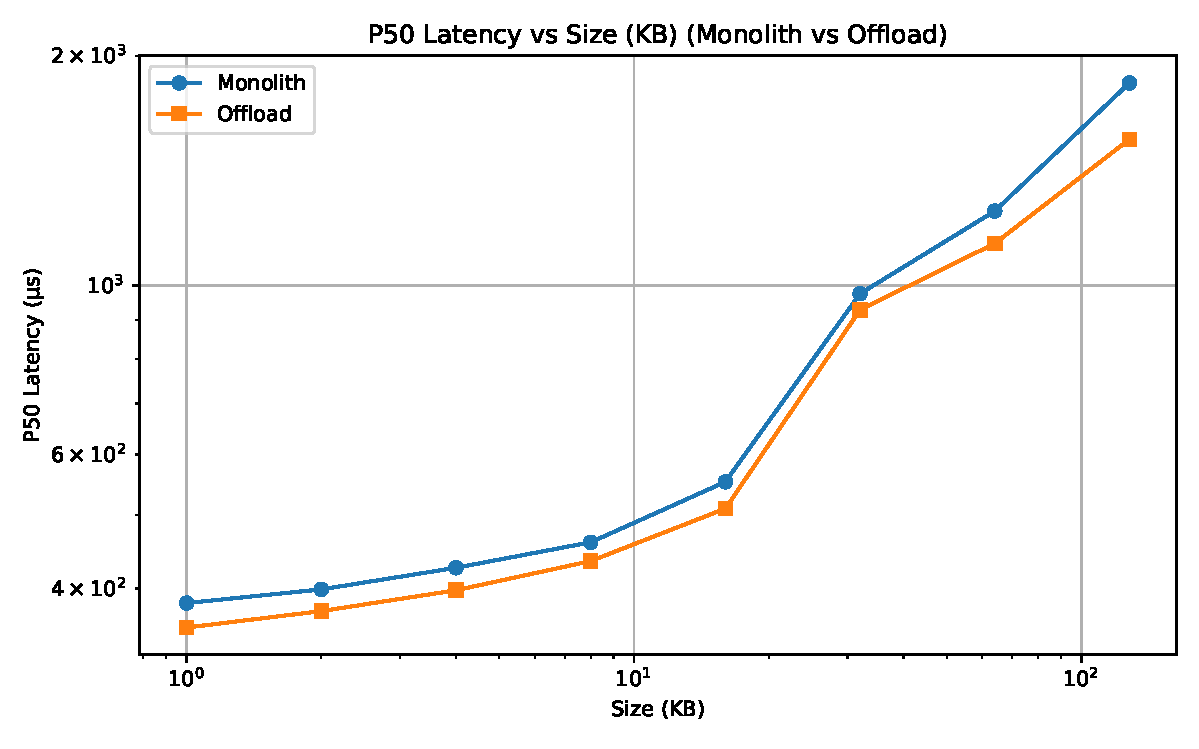
\includegraphics[width=0.48\textwidth]{size.pdf}%
  \hfill
  % second image:
  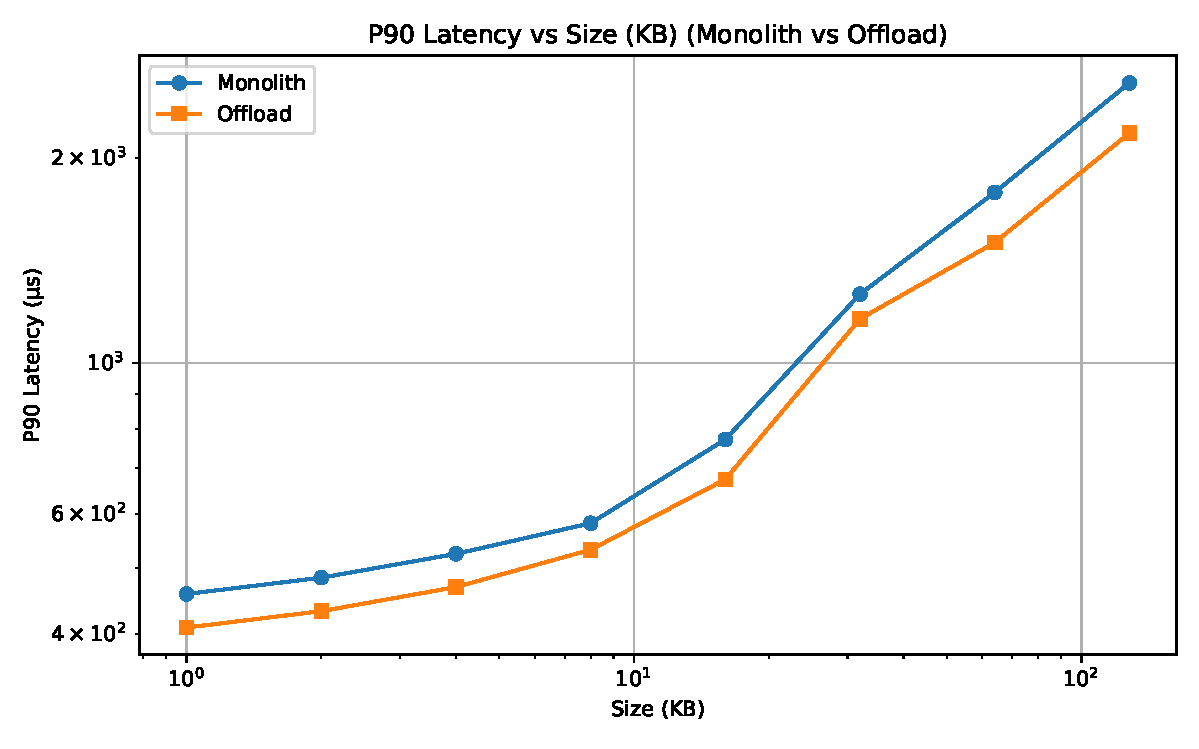
\includegraphics[width=0.48\textwidth]{size_p90.pdf}
  \caption{Median and 90th percentile latency versus the size of the input data. Sizes vary from 1KB to 128KB, with a data point at each power of two. Past 128KB, the latency increases by several orders of magnitude for both the monolithic configuration and the microservice (offload) configuration, so we omit those data points for clarity. The offered load is fixed at 4,000 requests per second. For both median and tail latency, the microservice configuration with offloaded (de)compression performs marginally better than the monolithic configuration.}
  \label{fig:size}
\end{figure*}

\begin{figure*}[!ht]            % “*”→span both columns; [!t]→force it to the top
  \centering
  % first image, take roughly half the page width:
  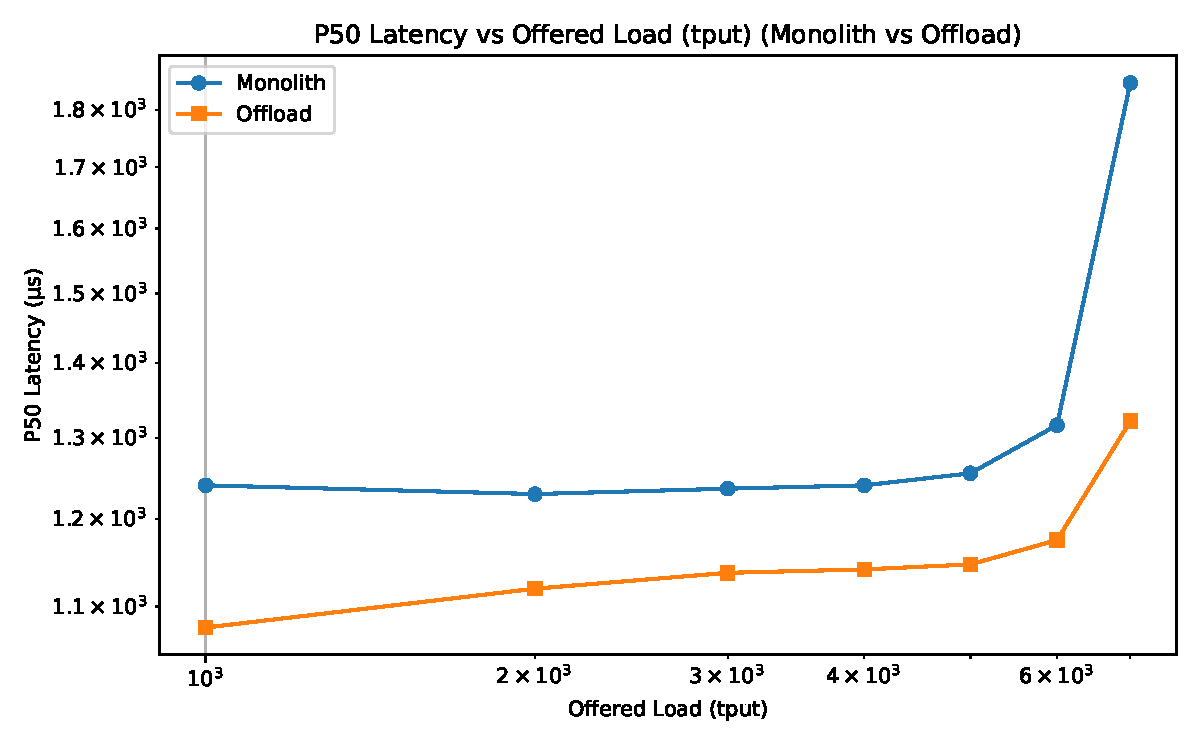
\includegraphics[width=0.48\textwidth]{p50.pdf}%
  \hfill
  % second image:
  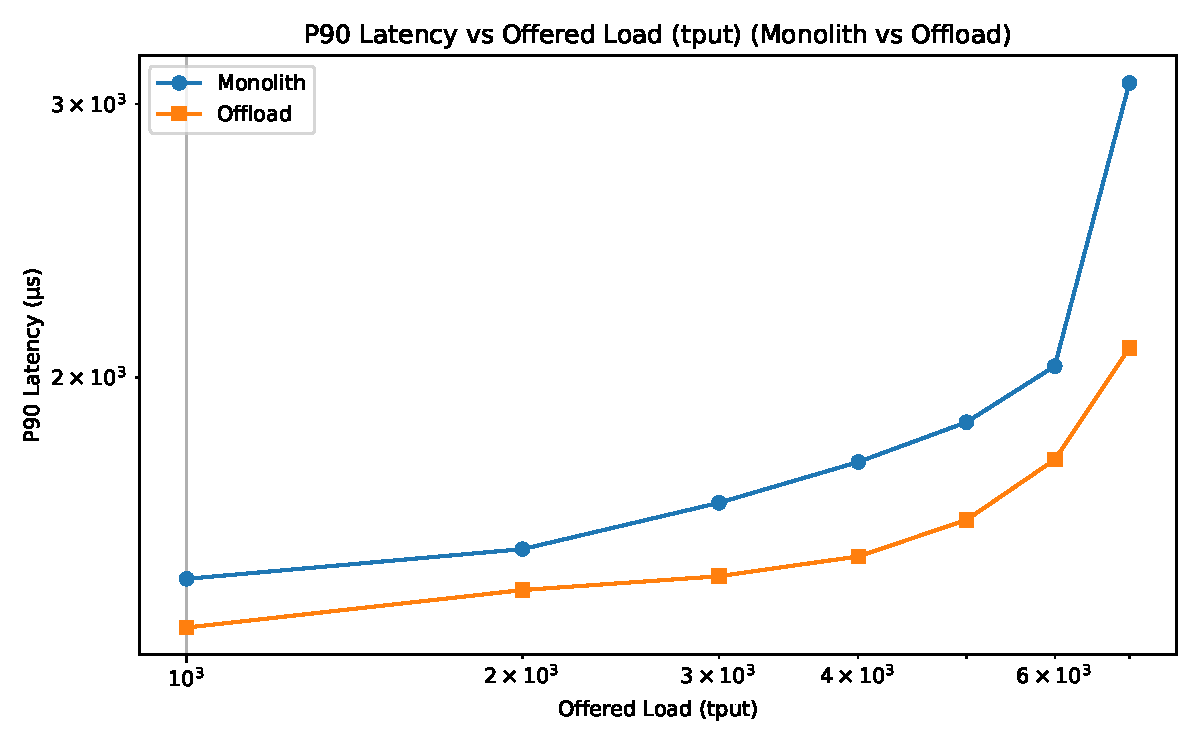
\includegraphics[width=0.48\textwidth]{p90.pdf}
  \caption{Median and 90th percentile latency versus the offered load. The load varies from 1,000 requests per second to 7,000. Past 7,000 requests per second, the latency increases by several orders of magnitude for both the monolithic configuration and the microservice (offload) configuration, so we omit those data points for clarity. The input data size is fixed at 64KB. Again, for both median and tail latency, the microservice configuration with offloaded (de)compression performs marginally better than the monolithic configuration.}
  \label{fig:tput}
\end{figure*}

\subsection{Experimental Setup}
We conduct experiments using one dual-socket server, each with a 28-core Intel Xeon Gold 5420+ CPU operating at 2.0 GHz and 256 GB of RAM. 
Hyperthreading was enabled. 
The operating system was Ubuntu 24.04. 
We pinned all containers to one socket, and we only used the IAA device local to the socket. 
The IAA was configured with 8 shared work queues and 8 engines.

\subsection{Service Configurations}
We evaluated two configurations for the compressed cache service.
\begin{enumerate}
  \item A monolithic configuration that places the frontend service and compression service in the same process and the same container. Communicating between the two services is done through a local function call. The QPL software path is used for (de)compression.
  \item A microservice configuration that splits the frontend service and compression service into separate containers, requiring that they communicate over gRPC, but offloading the (de)compression operations to the IAA.
\end{enumerate}
For both, we use Memcached as the cache implementation, which is hosted in its own container and accessed by the frontend service via gRPC. Likewise, the scheduler service is hosted in its own container and communicates with the compression service to collect operation metrics over gRPC.

For each service configuration, we run a microbenchmark that dispatches a configurable number of requests per second with a fixed request payload size. 
Using this microbenchmark, we measure the median and 90th percentile latency of the service under different request payload sizes and offered loads. 
By analyzing the difference in latencies, we can draw estimates of the tolerable network overhead for disaggregating an application into microservices across different hardware platforms. 
Though we run all services on the same server, we can easily extend our experiment to simulate network overhead by introducing artifial delays using Blueprint's latency injector plugin. 

\subsection{Size Variations}
Figure~\ref{fig:size} shows the median and 90th percentile latency of the two service configurations as a function of the request payload size. 
Promisingly, we find that the microservice configuration with offloaded (de)compression performs marginally better than the monolithic configuration for both median and tail latency, even though it incurs additional overhead from gRPC. 
For both median and tail latency, the microservice configuration sees improved latency on the order of low hundreds of microseconds.
For example, at 32KB, the median latency is 1.13ms for the microservice configuration and 1.25ms for the monolithic configuration, while the 90th percentile latency is 1.50ms for the microservice configuration and 1.78ms for the monolithic configuration. 
This seems to indicate that the network delay could reach 100 microseconds and it may still be worth splitting an application to take advantage of offload capabilities on remote servers.

\subsection{Load Variations}
Figure~\ref{fig:tput} shows the median and 90th percentile latency of the two service configurations as a function of the offered load.
Again, we find that the microservice configuration with offloaded (de)compression performs marginally better than the monolithic configuration for both median and tail latency, even with the additional overhead from gRPC.
The observed latency improvements are also similar to those in the size variation experiment, with the microservice configuration seeing improved latency on the order of low hundreds of microseconds across most of the offered load range.
However, notably, near peak load the median latency is 1.32ms for the microservice configuration and 1.85ms for the monolithic configuration, while the 90th percentile latency is 2.08ms for the microservice configuration and 3.09ms for the monolithic configuration.
This suggests a potentially significant benefit in the ability to absorb bursts of load in the microservice configuration.

\subsection{Takeaways}
The results of our experiments suggest that the microservice configuration with offloaded (de)compression can yield marginally better performance than the monolithic configuration, even when accounting for the additional overhead of gRPC communication and potential network delays. Our results indicate that location-aware scheduling that takes into account the network delay could be beneficial, but would require further investigation to quantify the trade-offs more precisely. The results would likely be even more promising with a high performance container networking interface (CNI) that minimizes the network overhead, such as Cilium~\cite{cilium}.
